\documentclass{article}
\usepackage[pdftex]{graphicx}
\usepackage{afterpage}
\usepackage{color,fancyvrb}
\usepackage[margin=1in]{geometry}
\usepackage[pdftex,bookmarks=true]{hyperref}   %Bookmarks


\title{Benchmark Agent Communication Language against communication using ActiveMQ}
\author{Avinash Joshi}
\usepackage{Sweave}
\begin{document}
\Sconcordance{concordance:ACLvsActiveMQ_Benchmark.tex:ACLvsActiveMQ_Benchmark.Rnw:%
1 10 1 1 0 53 1 1 17 4 0 1 2 2 1}

\maketitle
\begin{abstract}
This paper compares two methods of communication between agents/applications, Agent communication language(ACL) and Apache ActiveMQ. JADE inherently uses ACL for communication between it's agents. If an agent A is sending messages to agent B and the computation time of B is slower than the rate at which it receives messages from A, the inbox size of B which holds the unprocessed messages goes on increasing. This also increases the computation time of B. We explore an alternative way of sending messages namely ActiveMQ.
\end{abstract}

\section{Introduction}
Java Agent Development Framework or JADE is an agent development framework where agents are implemented in Java. It gives you an environment to execute your agents, class libraries to create agents and a monitoring toolkit. The agents use ACL for communicating and coordinating with each other.

\section{Field of study}
Find an effective method for communication between JADE agents. Benchmark the aforementioned two methods for number of messages consumed and the time difference between the message sent and message received.
\subsection{Hypothesis}
\begin{table}[htp]
\begin{tabular}{|l|l|}
\hline 
Communication Method & Hypothesis\tabularnewline
\hline 
\hline 
\multirow{1.ACL} &  \textbullet{} Does not need to push messages to an external application, the agent sending messages \\& should be faster and hence should send more messages\\&
\textbullet{}The result of the above point would be that the receiving agent will have it's inbox queued\\& and hence consumption of the message would be slower thereby\\& resulting in increase in computation time\tabularnewline
\hline
\multirow{2.ActiveMQ} & \textbullet{} Needs the agent to push messages to a queue.This should slow down the agent and\\& hence lesser number of messages will be sent.\\
&\textbullet{}The agent consuming the messages from the queue should be faster than the one\\& consuming from it's inbox as it is independent of the size.\tabularnewline
\hline
\end{tabular}
\end{table}

\section{Challenger Method}
ActiveMQ can also be used for JADE agents to communicate. This mode of communication challenges the conventional method of using the ACL communication which is built into the JADE framework.

\section{Experiment Details}
Two agents are used in this experiment. The first agent called \emph{LatSender} will send a message which has the time at which it is sent and the number of the message. The second agent called \emph{LatReceiver} will receive the message and log the time difference as soon as it gets it.

These two agents will communicate using both ACL and ActiveMQ and log their respective time differences. The results shall be later analyzed to see which mode of communication is better.

\section{Experiment Environment}
The agency is running on muESP which has the following configuration,
\begin{itemize}
\item OS - Ubuntu 12.04
\item Environment - Labs - Development Environment
\item muESP Build Version - 1.2.2S-3M-2C.4 
\item Number of core engines - 1
\item Number of machines in the R cluster - 4
\item Number of cores per machine - 4
\item RAM per machine - 12 GB
\item Number of active agencies - 8
\item Number of active agents - 29
\item Amount of time the bench-marking scripts were running - 135 mins
\end{itemize}
\clearpage

\section{Benchmark results}
%Loading libraries

\begin{table}[htp]
\begin{center}
\begin{tabular}{|l|l|l|}
\hline
&ACL & ActiveMQ\tabularnewline
\hline
Number of messages sent & 465000 & 26949\tabularnewline
\hline
Number of messages consumed & 9886 & 13563\tabularnewline
\hline
Number of messages in the queue & 455114 & 13386\tabularnewline
\hline
Percentage of messages consumed & 2.13\% & 50.33\%\tabularnewline
\hline
\end{tabular}
\end{center}
\end{table}

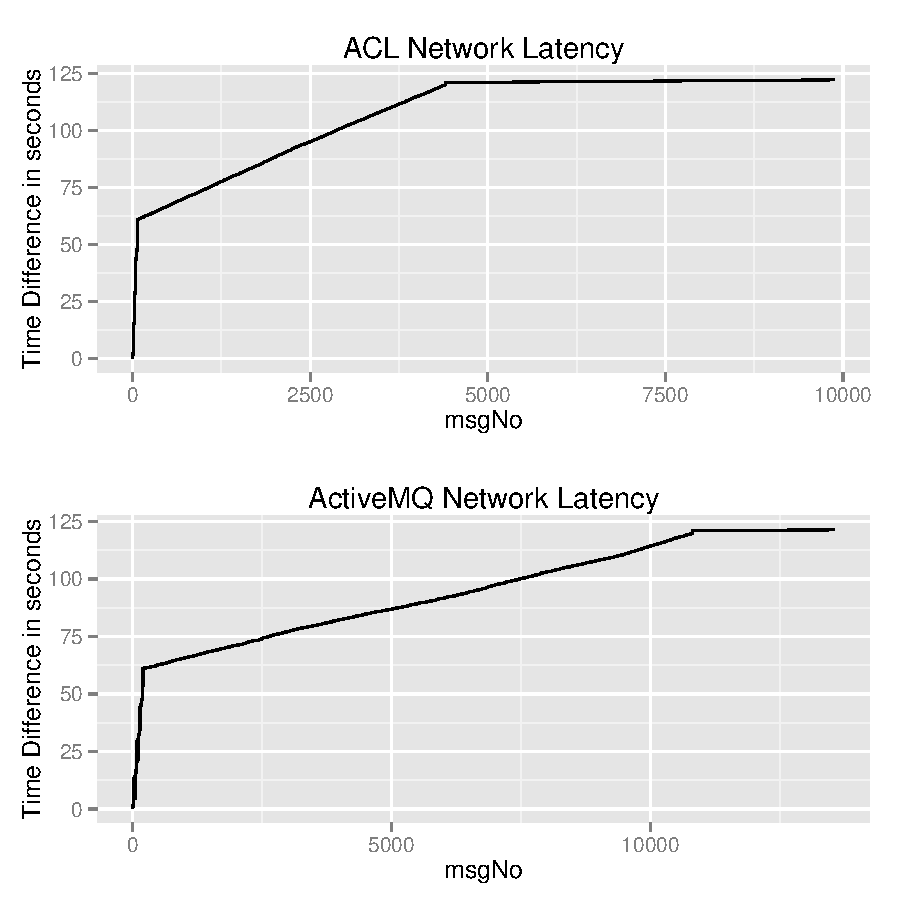
\includegraphics{ACLvsActiveMQ_Benchmark-002}
\clearpage

\section{Conclusion}
\begin{itemize}
\item Sending messages via ACL is faster than pushing messages to ActiveMQ
\item Inbox of an agent queues up faster in ACL communication affecting the agent's performance
\item The number of messages consumed via ActiveMQ is higher than ACL
\item The latency in the receiving agent getting the message is higher in ACL communication as compared to ActiveMQ

\textbf{In conclusion, if the agent sending messages is very fast, then ActiveMQ is a better option  otherwise ACL is the ideal choice.}
\end{itemize}

\section{References}
\begin{itemize}
\item \url{http://jade-lang.com/api/}
\item \url{http://en.wikipedia.org/w/index.php?title=Jade&oldid=570549171}
\item \url{http://en.wikipedia.org/w/index.php?title=Agent\_Communications\_Language&oldid=544223838}
\item \url{http://activemq.apache.org/maven/5.8.0/apidocs/index.html}
\end{itemize}
\end{document}
